\documentclass[11pt]{article}
\usepackage[margin=1in]{geometry}
\usepackage{fontspec}
\usepackage{booktabs}
\usepackage{longtable}
\usepackage{array}
\usepackage{graphicx}
\usepackage{adjustbox}
\usepackage[font=small,labelfont=bf]{caption}
\usepackage{natbib}
\usepackage{xurl}
\usepackage[hidelinks]{hyperref}
\usepackage{setspace}
\usepackage{amsmath}
\usepackage{placeins}
\setstretch{1.15}
\graphicspath{{../figs/}}
\newcommand{\CountRawRows}{5,817}
\newcommand{\CountExpandedRows}{5,861}
\newcommand{\CountRestoredRows}{44}
\newcommand{\CountRawPollIds}{2,565}
\newcommand{\CountDuplicatedPoliticianMonth}{1}
\newcommand{\CountPresidentialRows}{1,456}
\newcommand{\CountNonpresidentialRows}{4,405}
\newcommand{\CountMatchedDatedRows}{1,607}
\newcommand{\CountMainRows}{319}
\newcommand{\CountMainPolls}{306}
\newcommand{\CountMainPoliticians}{18}
\newcommand{\CountMainStates}{14}
\newcommand{\CountRawCatalogRows}{295}
\newcommand{\CountDistinctOffices}{251}
\newcommand{\CountDatedOffices}{89}
\newcommand{\CountCleanOffices}{161}
\newcommand{\CountUnmatchedNonpresidential}{76}
\newcommand{\CountIncompleteRows}{18}
\newcommand{\CountMainPreIn}{69.3}
\newcommand{\CountMainPreOut}{38.6}
\newcommand{\CountMainPostIn}{64.1}
\newcommand{\CountMainPostOut}{33.9}
\newcommand{\InEstimate}{-2.6}
\newcommand{\InLower}{-5.9}
\newcommand{\InUpper}{0.8}
\newcommand{\InP}{0.118}
\newcommand{\InDf}{11.0}
\newcommand{\OutEstimate}{-5.7}
\newcommand{\OutLower}{-10.0}
\newcommand{\OutUpper}{-1.5}
\newcommand{\OutP}{0.013}
\newcommand{\OutDf}{11.0}
\newcommand{\GapEstimate}{3.2}
\newcommand{\GapLower}{-0.1}
\newcommand{\GapUpper}{6.4}
\newcommand{\GapP}{0.058}
\newcommand{\GapDf}{11.0}
\newcommand{\InPenalty}{2.6}
\newcommand{\OutPenalty}{5.7}
\newcommand{\EqualEventChange}{2.1}
\newcommand{\EventMinChange}{-7.2}
\newcommand{\EventMaxChange}{22.6}
\newcommand{\LooMin}{2.2}
\newcommand{\LooMax}{3.9}
\newcommand{\NoTrendEstimate}{0.9}
\newcommand{\NoTrendLower}{-2.3}
\newcommand{\NoTrendUpper}{4.2}
\newcommand{\PlaceboEstimate}{-0.3}
\newcommand{\PlaceboLower}{-5.7}
\newcommand{\PlaceboUpper}{5.0}
\newcommand{\PlaceboOfficials}{14}
\newcommand{\LegacyInEstimate}{0.624}
\newcommand{\LegacyOutEstimate}{-3.140}
\newcommand{\LegacyGapEstimate}{3.763}
\newcommand{\LegacyN}{1,476}
\newcommand{\RestoredMain}{4}
\newcommand{\BootstrapP}{0.063}
\newcommand{\BootstrapDraws}{9,999}
\newcommand{\SupportedEstimate}{0.8}
\newcommand{\SupportedLower}{-3.8}
\newcommand{\SupportedUpper}{5.3}
\newcommand{\SupportedOfficials}{8}
\newcommand{\PairedEstimate}{1.6}
\newcommand{\PairedLower}{-2.0}
\newcommand{\PairedUpper}{5.2}
\newcommand{\PairedPoliticians}{10}
\newcommand{\PairedStates}{8}
\newcommand{\PairedUnits}{12}
\newcommand{\PairedN}{211}
\newcommand{\TreatedEstimate}{2.7}
\newcommand{\TreatedLower}{-1.2}
\newcommand{\TreatedUpper}{6.5}
\newcommand{\TreatedPoliticians}{10}
\newcommand{\TreatedStates}{8}
\newcommand{\TreatedUnits}{12}
\newcommand{\TreatedN}{211}
\newcommand{\RepeatedEstimate}{2.7}
\newcommand{\RepeatedLower}{-0.3}
\newcommand{\RepeatedUpper}{5.7}
\newcommand{\RepeatedPoliticians}{19}
\newcommand{\RepeatedStates}{14}
\newcommand{\RepeatedUnits}{21}
\newcommand{\RepeatedN}{349}
\newcommand{\CorrectedEstimate}{3.8}
\newcommand{\CorrectedLower}{0.9}
\newcommand{\CorrectedUpper}{6.7}
\newcommand{\CorrectedPoliticians}{18}
\newcommand{\CorrectedStates}{14}
\newcommand{\CorrectedN}{319}
\newcommand{\LargestMainPenalty}{5.9}
\newcommand{\LargestSupportedPenalty}{8.6}
\newcommand{\LegacyClusterInLower}{-6.2}
\newcommand{\LegacyClusterInUpper}{7.4}
\newcommand{\LikeInEstimate}{-2.6}
\newcommand{\LikeInRatio}{5.2}
\newcommand{\LikeInP}{0.069}
\newcommand{\LikeOutEstimate}{-5.2}
\newcommand{\LikeOutRatio}{472.7}
\newcommand{\LikeOutP}{0.000}
\newcommand{\LikeGapEstimate}{3.0}
\newcommand{\LikeGapRatio}{6.0}
\newcommand{\LikeGapP}{0.058}
\newcommand{\InteractionP}{0.058}
\newcommand{\InteractionDirectionalP}{0.029}
\newcommand{\InteractionDirectionalLower}{0.5}
\newcommand{\BootstrapDirectionalP}{0.032}

\newcommand{\InventoryRows}{295}
\newcommand{\InventoryDatedRows}{132}
\newcommand{\InventoryCleanRows}{162}
\newcommand{\InventoryIncompleteRows}{1}
\newcommand{\InventoryDistinctDates}{130}
\newcommand{\InventoryDatedOffices}{89}
\newcommand{\InventoryValidDatedOffices}{88}
\newcommand{\InventoryMissingIdentity}{1}
\newcommand{\InventoryOutsidePeriod}{2}
\newcommand{\InventoryMainEvents}{18}
\newcommand{\InventoryCorruption}{12}
\newcommand{\InventorySexual}{1}
\newcommand{\InventoryRepublican}{13}
\newcommand{\InventoryDemocrat}{5}
\newcommand{\InventorySenators}{12}
\newcommand{\InventoryGovernors}{6}
\newcommand{\InventoryOlympicOnsets}{3}
\newcommand{\InventoryOlympicMain}{0}
\newcommand{\OverallEstimate}{-4.2}
\newcommand{\OverallLower}{-8.43}
\newcommand{\OverallUpper}{-0.04}

\newcommand{\ExpStrongControlEstimate}{10.2}
\newcommand{\ExpStrongControlLower}{4.5}
\newcommand{\ExpStrongControlUpper}{15.9}
\newcommand{\ExpStrongControlP}{<.001}
\newcommand{\ExpStrongResponseEstimate}{5.9}
\newcommand{\ExpStrongResponseLower}{0.5}
\newcommand{\ExpStrongResponseUpper}{11.2}
\newcommand{\ExpStrongResponseP}{.031}
\newcommand{\ExpModerationControlEstimate}{12.2}
\newcommand{\ExpModerationControlLower}{5.3}
\newcommand{\ExpModerationControlUpper}{19.1}
\newcommand{\ExpModerationControlP}{<.001}
\newcommand{\ExpModerationResponseEstimate}{6.0}
\newcommand{\ExpModerationResponseLower}{-0.6}
\newcommand{\ExpModerationResponseUpper}{12.6}
\newcommand{\ExpModerationResponseP}{.076}
\newcommand{\ExpAssignedN}{746}
\newcommand{\ExpStrongN}{226}
\newcommand{\ExpAttentionN}{724}
\newcommand{\ExpAttentionStrongN}{223}
\newcommand{\ExpArchivedInteractionEstimate}{11.2}
\newcommand{\ExpArchivedInteractionLower}{4.1}
\newcommand{\ExpArchivedInteractionUpper}{18.3}
\newcommand{\ExpArchivedInteractionP}{.002}
\newcommand{\ExpDirectOwnTraitsEstimate}{8.9}
\newcommand{\ExpDirectOwnTraitsLower}{2.3}
\newcommand{\ExpDirectOwnTraitsUpper}{15.6}
\newcommand{\ExpDirectOwnTraitsP}{.009}
\newcommand{\ExpDirectOpponentTraitsEstimate}{-2.8}
\newcommand{\ExpDirectOpponentTraitsLower}{-9.0}
\newcommand{\ExpDirectOpponentTraitsUpper}{3.3}
\newcommand{\ExpDirectOpponentTraitsP}{.362}

\newcommand{\ResearchMilestones}{39}
\newcommand{\ResearchEpisodes}{30}
\newcommand{\ResearchOfficials}{28}
\newcommand{\ResearchSearched}{32}
\newcommand{\ResearchCoreMilestones}{27}
\newcommand{\AnesPaired}{2501}
\newcommand{\AnesWeighted}{2065}
\newcommand{\AnesSameDay}{52}
\newcommand{\PreussEvents}{218}
\newcommand{\PreussMatched}{27}
\newcommand{\NyhanEpisodes}{45}
\newcommand{\NyhanMatched}{18}
\newcommand{\NyhanOnsets}{43}
\newcommand{\NyhanArticles}{436}
\newcommand{\RakichRows}{275}
\newcommand{\RakichMatched}{18}

\newcommand{\PublicityPrograms}{146}
\newcommand{\PublicitySegments}{29}
\newcommand{\OlympicMinutesABC}{2.9}
\newcommand{\AwareABC}{65.7}
\newcommand{\OlympicMinutesCBS}{1.0}
\newcommand{\AwareCBS}{67.0}
\newcommand{\OlympicMinutesNBC}{7.2}
\newcommand{\AwareNBC}{66.9}
\newcommand{\PublicityPresenceEstimate}{2.06}
\newcommand{\PublicityPresenceLower}{-28.12}
\newcommand{\PublicityPresenceUpper}{32.24}
\newcommand{\PublicityDurationEstimate}{-0.45}
\newcommand{\PublicityDurationLower}{-1.36}
\newcommand{\PublicityDurationUpper}{0.46}
\newcommand{\PublicityInterviews}{15,109}
\newcommand{\PublicityNetworkViewers}{7,831}
\newcommand{\PublicityPartisanRatings}{5,067}

\newcommand{\TableStyle}{\small\setlength{\tabcolsep}{5pt}\renewcommand{\arraystretch}{1.12}}
\title{Partisan Asymmetry in Responses to Scandal}
\author{Douglas J. Ahler \and Gaurav Sood}
\date{Working draft: October 2026}
\begin{document}
\maketitle
\begin{abstract}
\noindent Approval declines after political scandals, with greater losses among opposing partisans. Across \CountMainPoliticians{} governors and senators, co-partisan approval falls by \InPenalty{} percentage points and opposing-partisan approval by \OutPenalty{} points. The partisan difference is \GapEstimate{} points (95\% confidence interval [\GapLower, \GapUpper]; directional $p=\InteractionDirectionalP$). These changes indicate modest average penalties and some partisan protection, although the size of the difference varies with event dating and trend adjustment. During the 2004 Swift Boat controversy, audiences reported similar awareness across networks just after the Olympics opened, despite much greater Olympic coverage on NBC. A separate survey experiment examines how citizens judge partisans who maintain support for a leader after controversy. Among strong partisans, a portrayal of opponents retaining rather than withdrawing support increases a rescaled trait-polarization index by \ExpStrongResponseEstimate{} points [\ExpStrongResponseLower, \ExpStrongResponseUpper]. Together, the results connect partisan differences in accountability to citizens' evaluations of their political opponents.
\end{abstract}

\section{Introduction}

Political accountability requires citizens to judge what their representatives do. Partisanship can complicate that judgment. A citizen may excuse an ally's misconduct, discount the accusation, or continue to approve of the politician despite accepting it. The same citizen may take a similar accusation against an opponent as further reason for disapproval. These possibilities imply an asymmetry in responses to scandal, but they do not all imply an absence of accountability within the politician's party.

The distinction matters empirically. A politician can lose support among both groups while losing more among opponents. Conversely, one estimate can be distinguishable from zero and another indistinguishable from zero even when the difference between them is poorly determined. The relevant comparison is the change among co-partisans minus the change among opposing partisans, measured for the same politician in the same polls. We estimate that comparison directly.

We combine repeated approval polls of governors and senators with a catalog of public controversies between 2005 and 2011. Comparing Democrats and Republicans within the same polls holds the politician and political moment constant. The main analysis follows each official around the first cataloged event and estimates the difference between co-partisan and opposing-partisan approval changes.

Co-partisan approval falls by \InPenalty{} percentage points, compared with \OutPenalty{} points among opposing partisans. The difference of \GapEstimate{} points supports the predicted partisan asymmetry ($p=\InteractionDirectionalP$, one-sided). The co-partisan interval excludes a ten-point average loss while permitting losses of roughly \LargestMainPenalty{} points. Party loyalty thus provides some protection against punishment, but the observed losses remain consequential in a close electoral contest. The magnitude of the partisan difference depends on the event dates and counterfactual trend.

Scandal responses can also affect relations between ordinary citizens. In a survey experiment, strong partisans evaluate the parties more differently after learning that opponents maintained their support for a leader following controversy. The experiment connects perceived accountability to partisan evaluations, complementing the evidence on approval of political leaders.

A study of the 2004 Swift Boat controversy examines whether competing Olympic news reduced publicity. NBC devoted substantially more evening-news time to the Olympics than ABC or CBS, yet continued to cover the allegations. Its viewers reported similar awareness of the advertisement. This comparison connects the attention mechanism to observed coverage and audience knowledge.

\section{Scandal, Partisanship, and Accountability}

A scandal can reveal information about a politician's conduct, competence, or honesty. Whether that information changes an evaluation depends partly on what a citizen believed before hearing it and how much weight the citizen gives the conduct. \citet{stoker1993}, for example, shows that reactions to Gary Hart's scandal varied with prior predispositions and the considerations citizens brought to candidate evaluation. A common accusation need not produce a common change in opinion.

Exposure can differ as well. \citet{puglisi2011} find that newspapers' partisan leanings predict their relative coverage of Democratic and Republican scandals. If people encounter different accounts, an asymmetry in approval need not arise solely from different processing of identical information. Our approval records measure neither exposure nor the credibility citizens assign to an allegation. They cannot separate these explanations.

Approval also differs from electoral choice. A citizen can disapprove of an incumbent and still prefer that incumbent to the opposing party's candidate. \citet{eggers2014} studies this tradeoff in the British expenses scandal, relating electoral accountability to the partisan stakes of a contest. Our outcome is job approval, not a vote or a willingness to replace the officeholder. An approval penalty is evidence of a less favorable evaluation, but not necessarily evidence of electoral punishment.

The broader literature finds adverse but variable consequences. \citet{basinger2013} documents electoral losses and departures after congressional scandals, while \citet{praino2022} synthesize evidence of electoral punishment. \citet{sikorski2018} emphasizes variation across scandal types, prior attitudes, and contexts, as well as the limited measurement of news intensity. These findings make the definition and composition of a scandal inventory part of the substantive question.

Experimental evidence also distinguishes partisan protection from indifference to misconduct. \citet{anduiza2013} finds partisan bias in corruption judgments, and \citet{lee2023} studies partisan forgiveness in the Trudeau blackface controversy. \citet{funck2022} shows that voters can judge a politician's morality negatively while preferring the politician's party or policies. Conversely, \citet{onishi2026} finds governing-party supporters withdrawing support after well-substantiated Partygate revelations. A universal claim of co-partisan immunity would miss these differences in information and context.

The baseline levels deserve attention. In the main sample's pre-event polls, average co-partisan approval is \CountMainPreIn\%, compared with \CountMainPreOut\% among opposing partisans. Opposing-partisan approval is lower, but far from universally at its lower bound. Both groups have room to downgrade an official. These are averages of aggregate poll percentages. They are not estimates of the proportion of all American Democrats or Republicans who approve of the officials, and the difference between regression intercepts is not their substitute.

\section{Data and Comparisons}

\subsection{Approval records}

The approval series contains \CountRawRows{} politician-poll records and \CountRawPollIds{} historical poll identifiers. A poll can rate more than one politician, so records, polls, and respondents are different units. The data contain presidents, senators, and governors; the scandal catalog supplies office-specific entries for senators and governors. Presidential ratings are therefore outside the analysis.

The approval data combine the Jacobson series with SurveyUSA polls. Source records supply \CountRestoredRows{} senator and governor observations from December 2006 in addition to those in the initial combined series; \RestoredMain{} fall within the main event windows. The replication materials preserve the source files and their correspondence to the combined panel.

The later SurveyUSA records supply fieldwork dates, original poll identifiers, overall sample sizes, and rounded partisan composition shares. The earlier files identify months rather than exact interview dates. Neither source supplies exact partisan subgroup denominators throughout the panel. We consequently give each politician-poll observation equal weight, rather than assigning spurious binomial precision to percentages. A sensitivity gives each politician equal total weight. California poll 17884 separately categorizes strong and weak partisans; its unpooled party columns are not comparable with the usual party categories and are excluded from analysis. This exclusion does not remove a main-sample event.

For a Democratic officeholder, co-partisan approval is approval among Democrats and opposing-partisan approval is approval among Republicans. The definitions reverse for a Republican officeholder. We retain only rows with both outcomes and a known major-party affiliation. The paired difference preserves the covariance of the two approval measures. Missing percentages remain missing.

\subsection{Recorded scandals}

Following \citet{hayes2025}, we define a scandal as a public allegation that an elected official broke the law or seriously violated a widely held ethical or social norm. The allegation, rather than a finding of guilt, defines the event. We extend this definition to allegations involving the official's campaign, staff, or administration, recording organizational involvement separately from alleged personal misconduct. Ordinary policy disagreement or an unpopular decision alone does not qualify. Like Hayes, we impose no minimum amount of news coverage: publicity is a variable whose consequences we seek to study. This differs from the media-recognition approach of \citet{nyhan2017}, which identifies scandals through their treatment in the press.

For the expanded inventory, a dated source must identify the alleged conduct, the norm or legal obligation at issue, and the person or organization involved. Connected allegations constitute one episode; initial reports, new evidence, indictments, apologies, and clearances are dated milestones within it. A later clearance does not erase the earlier public allegation. We retain offensive remarks, association-only controversies, and other cases without an identified breach as a broader comparison category, and flag unresolved allegations or dates for further review. These rules govern the extension. The estimates reported below use the historical catalog, whose broader definition also includes inflammatory statements and incompetence.

The scandal file contains \CountRawCatalogRows{} coding rows. It distinguishes sexual misconduct, corruption or misuse of office, racist or inflammatory statements, incompetence, and other categories; it also contains records coded ``clean.'' Multiple rows can concern the same official or different aspects of the same episode. We match on state, office, and normalized surname, distinguishing John and Mark Warner using their party records. Name suffixes are removed explicitly. Unmatched or incompletely coded officials are not recoded as clean.

The timing variable warrants particular care. The codebook asks when a scandal first became public, but several entries instead mark a later report, indictment, or other development. The date review in the replication materials records the supporting evidence and uncertainty. For example, a Justice Department report concerning the dismissal of a U.S. attorney was publicly released in September 2008, whereas the Kit Bond entry is dated November.\footnote{The release and report are available from the \href{https://www.justice.gov/archive/opa/pr/2008/September/08-opa-859.html}{Department of Justice} and its \href{https://oig.justice.gov/sites/default/files/archive/special/s0809a/chapter4.htm}{Office of the Inspector General}.} Other entries concern allegations publicly discussed before the recorded month. A date recorded with daily precision need not identify the onset of public knowledge.

The main specification therefore uses the first \emph{cataloged} event for an official and describes changes around that recorded date. It does not treat every event as the first disclosure of misconduct. We separately examine source-supported alternative dates and repeated recorded events. Neither exercise reconstructs a complete history of what each respondent could have learned.

External inventories provide independent checks with different measurement rules. The congressional data of \citet{preuss2024} distinguish the first report located in a news database from subsequent major-newspaper coverage and retain article references. The governor data of \citet{nyhan2017} identify media recognition under an explicit Associated Press coding rule. Their dates are preserved under those definitions in the replication materials. Selecting only episodes that attain substantial coverage would condition on publicity, a consequential restriction when studying news congestion.

The inventory contains \InventoryDatedRows{} dated coding rows, \InventoryCleanRows{} clean entries, and \InventoryIncompleteRows{} incomplete entry. The dated rows form \InventoryDistinctDates{} distinct official-date combinations; these are not necessarily independent episodes. One Rubio entry lacks state and office, and \InventoryOutsidePeriod{} dates fall outside the codebook's stated period. The main sample is much narrower: \InventoryRepublican{} Republicans and \InventoryDemocrat{} Democrats, comprising \InventorySenators{} senators and \InventoryGovernors{} governors. Of its \InventoryMainEvents{} first events, \InventoryCorruption{} concern corruption or misuse of office. No prostitution or sexual-assault case enters the main comparison. Appendix Table~\ref{tab:inventory} compares the full category mix with the retained events. The replication inventory identifies each official's polling support and unresolved coding issues.

\subsection{Analytic window}

The main window includes up to twelve months before and twelve months after the first cataloged event, omitting the event month. An official must have at least two usable polls on each side. We stop before the month of the next cataloged event and retain the official's event-party affiliation. These rules reduce contamination by overlapping episodes and avoid treating officials observed on only one side as informative before/after comparisons. They also select on available follow-up: scandals followed by resignation, electoral defeat, or discontinued polling may be poorly represented.

The resulting sample contains \CountMainRows{} records from \CountMainPolls{} source polls for \CountMainPoliticians{} officials in \CountMainStates{} states. Appendix Table~\ref{tab:support} identifies every official, event date, and number of pre- and post-event observations. A fieldwork-based sensitivity retains event-month polls only when their entire known interview window falls strictly before or strictly after the recorded event. Polls spanning that date, or with an unknown end date, do not receive a precise pre/post classification.

\section{Estimation and Interpretation}

For each approval measure, we estimate
\begin{equation}
Y_{it}=\alpha_i+\beta\,\mathrm{Post}_{it}+\gamma r_{it}+\varepsilon_{it},
\label{eq:model}
\end{equation}
where $i$ identifies a politician-office, $r_{it}$ is the number of calendar months from the recorded event, and $\mathrm{Post}_{it}$ indicates a later month. The official fixed effects absorb stable differences in approval levels. The common linear trend allows approval to be changing before the event. The coefficient $\beta$ is the fitted level shift relative to that trend, not the unadjusted difference between all observations before and after the event.

We estimate the same equation for $G_{it}=Y^{\mathrm{co}}_{it}-Y^{\mathrm{opposing}}_{it}$. With the same rows and regressors, its post-event coefficient equals the co-partisan coefficient minus the opposing-partisan coefficient. A positive value means that co-partisan approval declines less, or rises more. This direct comparison supplies the test of asymmetry; separate significance tests cannot supply it. The archived hypothesis predicts a larger penalty among opposing partisans. We therefore test $H_0:\beta_G\leq 0$ against $H_1:\beta_G>0$ for the gap, while also reporting two-sided probabilities and 95\% two-sided intervals. This is the directional hypothesis motivating the study; the specification and sensitivity analyses are retrospective.

Uncertainty allows arbitrary dependence within states, including repeated observations of an official and correlated assessments of different officials in the same state. We use the CR2 covariance adjustment and coefficient-specific Satterthwaite degrees of freedom \citep{pustejovsky2018}. The main contrast has approximately \GapDf{} effective degrees of freedom. Politician clustering and a restricted wild cluster bootstrap provide additional checks. State clustering still assumes independence across states conditional on the fitted model. National party-specific shocks can violate that assumption; calendar-month effects probe part of this concern.

A causal interpretation would require the approval trajectory absent the scandal to follow the specified counterfactual, with no simultaneous cause of a discontinuity, relevant anticipation, or changing sample composition. Earlier revelations, concurrent campaign developments, and selective follow-up can violate these conditions. We interpret the estimates as adjusted changes around recorded events and assess their sensitivity to event dates, trends, and comparison samples.

\section{Results}

\subsection{Approval levels and the partisan difference}

The fitted decline in approval is larger among opposing partisans. Co-partisan approval also has a negative point estimate. Table~\ref{tab:main} estimates a co-partisan change of \InEstimate{} points and an opposing-partisan change of \OutEstimate{} points. Their difference is \GapEstimate{} points [\GapLower, \GapUpper]. The co-partisan interval is compatible with a substantively meaningful decline. The directional test supports greater opposing-partisan punishment ($p=\InteractionDirectionalP$). The two-sided interval spans approximate equality through a several-point widening of the approval gap; the 95\% one-sided lower bound is \InteractionDirectionalLower{} points.

\begin{table}[htbp]
\centering\TableStyle
\caption{Approval changes around the first cataloged scandal.}
\label{tab:main}
\begin{tabular}{lrrrrr}
\toprule
Outcome & Change & SE & 95\% CI & df & $p$ \\
\midrule
Co-partisan approval & -2.6 & 1.5 & [-5.9, 0.8] & 11.0 & 0.118 \\
Opposing-partisan approval & -5.7 & 2.0 & [-10.0, -1.5] & 11.0 & 0.013 \\
Co-partisan minus opposing & 3.2 & 1.5 & [-0.1, 6.4] & 11.0 & 0.058 \\
\bottomrule
\end{tabular}

\begin{minipage}{\linewidth}\footnotesize
\emph{Note}: Percentage-point coefficients on the post-event indicator in Equation~\ref{eq:model}. Same \CountMainRows{} politician-poll observations in all rows. Official fixed effects and a common linear month trend; equal record weights. CR2 standard errors clustered by state; 95\% confidence intervals and two-sided tests use Satterthwaite degrees of freedom. The final row tests the difference directly.
\end{minipage}
\end{table}

The fitted contrast should not be confused with the raw pooled change. Average co-partisan approval moves from \CountMainPreIn\% before the event to \CountMainPostIn\% afterward; opposing-partisan approval moves from \CountMainPreOut\% to \CountMainPostOut\%. The composition of officials and observation times differs between those pooled averages. Giving each official equal weight, the average within-official change in the raw approval gap is \EqualEventChange{} points. Neither calculation adjusts for an ongoing trend. The no-trend fixed-effects estimate is \NoTrendEstimate{} points [\NoTrendLower, \NoTrendUpper], compared with \GapEstimate{} in the main model. Detrending is consequential, not a routine cosmetic adjustment.

\begin{figure}[htbp]
\centering
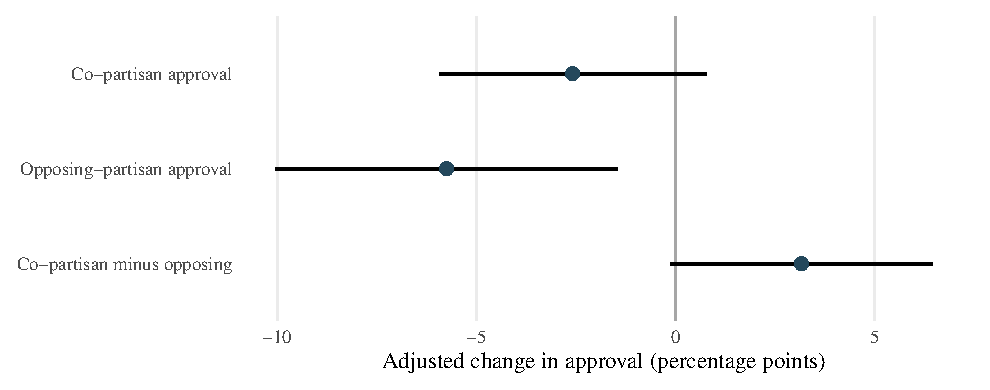
\includegraphics[width=\linewidth]{approval_changes.pdf}
\caption{Adjusted approval changes and their uncertainty. Points are the three post-event coefficients in Table~\ref{tab:main}; horizontal lines are state-clustered CR2 95\% confidence intervals using Satterthwaite degrees of freedom. Positive values in the final row indicate a widening co-partisan minus opposing-partisan approval gap.}
\label{fig:main}
\end{figure}

\subsection{What effect sizes do the estimates exclude?}

The intervals are informative about magnitude even where they include zero. The main co-partisan interval excludes a ten-point approval loss, while allowing losses as large as about \LargestMainPenalty{} points. A five-point penalty remains compatible with the main estimate. Table~\ref{tab:bounds} uses two-, five-, and ten-point penalties as transparent comparison values, not as preregistered thresholds for importance. The no-trend and better-supported-date analyses likewise exclude a ten-point co-partisan loss, but do not exclude a five-point loss. Thus the evidence weighs against large average co-partisan penalties in these samples; it cannot establish that their response is negligible.

\begin{table}[htbp]
\centering\TableStyle
\caption{Co-partisan penalties excluded or retained by the intervals.}
\label{tab:bounds}
\adjustbox{max width=\linewidth}{\begin{tabular}{llccc}
\toprule
Specification & 95\% interval & $-2$ points & $-5$ points & $-10$ points \\
\midrule
Primary: 12 months & [-5.9, 0.8] & Included & Included & Excluded \\
No time trend & [-6.6, 1.2] & Included & Included & Excluded \\
Supported exposure months & [-8.6, -0.7] & Included & Included & Excluded \\
\bottomrule
\end{tabular}
}
\begin{minipage}{\linewidth}\footnotesize
\emph{Note}: A negative change is a decline in approval. ``Excluded'' means the specified penalty lies below the lower endpoint of the pointwise 95\% CR2/Satterthwaite interval; ``included'' means it lies inside that interval. These are comparisons with the reported confidence sets, not tests that an effect is exactly zero or a preregistered equivalence margin. Units are percentage points.
\end{minipage}
\end{table}

The direct partisan contrast also constrains the interpretation. Its main interval, [\GapLower, \GapUpper], excludes a substantial asymmetry in which co-partisans punish more than opponents. It permits approximate equality and appreciably greater punishment by opposing partisans. Among the better-supported events, [\SupportedLower, \SupportedUpper], even a five-point asymmetry in the reverse direction lies outside the interval, although smaller reversals remain possible. These results support a directional account of partisan asymmetry more than a claim of precisely zero co-partisan accountability.

\subsection{The interaction and likelihood support}

The paired-gap regression is also an interaction test. Stacking the two approval outcomes and interacting co-partisan status with the post-event indicator, the time trend, and the official fixed effects reproduces the main estimate, standard error and directional probability (\InteractionDirectionalP; two-sided \InteractionP). The full set of interactions permits different baseline levels and trends for each partisan group. The post-by-co-partisan coefficient is the difference in their fitted approval changes.

A likelihood analysis asks which magnitudes the data favor, rather than classifying the result solely by a probability cutoff. We fit Gaussian generalized least squares models with the same mean specification and continuous AR(1) residual correlation within officials. We use maximum likelihood, re-estimating the correlation, residual variance and remaining coefficients at each candidate post-event effect. This model assumes a common residual variance and correlation parameter for each outcome, and independence across officials. These are stronger covariance assumptions than state-clustered inference.

The gap likelihood peaks at \LikeGapEstimate{} points and is \LikeGapRatio{} times as high there as at zero. Its likelihood-ratio test gives a two-sided probability of \LikeGapP. For co-partisan approval, the peak is a \LikeInEstimate{}-point change, with likelihood \LikeInRatio{} times as high as at zero; the opposing-partisan peak is \LikeOutEstimate{} points. Figure~\ref{fig:likelihood} makes the substantive comparison visible: the data favor a smaller co-partisan penalty and give little support to a large co-partisan loss or a large reverse asymmetry. The co-partisan likelihood does not peak at zero. These are profile-likelihood ratios under the stated model, not posterior probabilities or Bayes factors, and they do not average over uncertain event dates.

\begin{figure}[htbp]
\centering
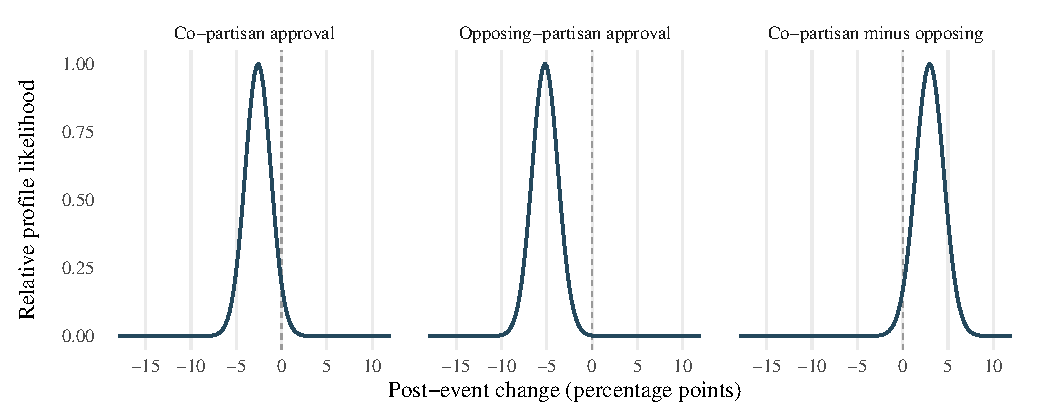
\includegraphics[width=\linewidth]{likelihood_profiles.pdf}
\caption{Likelihood support for approval changes. Each curve profiles the Gaussian likelihood over the post-event coefficient, re-estimating nuisance parameters under within-official continuous AR(1) correlation. Each maximum is normalized to one. The vertical reference is zero. Curves show relative likelihood, not probability densities; inference assumes independent officials and the specified Gaussian covariance model. Same main sample as Table~\ref{tab:main}.}
\label{fig:likelihood}
\end{figure}

\subsection{How much depends on the specification?}

The estimated partisan difference is positive across the specifications in Table~\ref{tab:sensitivity}, but its precision changes. Shorter and longer windows alter both the time horizon and usable observations. Assigning the whole event month to the pre- or post-period makes different assumptions about exposure; known fieldwork dates provide a more informative check where available. Separate pre/post trends and politician-specific trends relax the main model's common-slope restriction. The calendar-month specification controls for shared calendar shocks, but is still an observational comparison among selected, eventually affected officials, not a design that establishes a causal effect.

\begin{table}[htbp]
\centering\TableStyle
\caption{Sensitivity of the estimated partisan difference.}
\label{tab:sensitivity}
\adjustbox{max width=\linewidth}{\begin{tabular}{lrrrr}
\toprule
Specification & Gap change & 95\% CI & Rows & Officials \\
\midrule
Primary: 12 months & 3.2 & [-0.1, 6.4] & 319 & 18 \\
Fieldwork-date classification & 2.8 & [-0.5, 6.2] & 327 & 18 \\
Original coverage only & 3.0 & [-0.3, 6.3] & 315 & 18 \\
6 months & 2.3 & [-2.0, 6.7] & 190 & 18 \\
18 months & 2.9 & [0.0, 5.7] & 405 & 18 \\
No censoring at later scandals & 3.5 & [0.3, 6.6] & 341 & 19 \\
Event month assigned post & 3.4 & [0.6, 6.3] & 349 & 19 \\
Event month assigned pre & 1.8 & [-1.1, 4.6] & 350 & 19 \\
Separate pre/post slopes & 3.3 & [-0.1, 6.8] & 319 & 18 \\
Politician-specific slopes & 2.5 & [-1.0, 6.1] & 319 & 18 \\
Calendar-month fixed effects & 4.5 & [0.6, 8.4] & 319 & 18 \\
Politician clustering & 3.2 & [-0.1, 6.5] & 319 & 18 \\
No time trend & 0.9 & [-2.3, 4.2] & 319 & 18 \\
Equal politician weight & 3.1 & [0.2, 6.0] & 319 & 18 \\
One observation per side & 2.8 & [-0.2, 5.9] & 355 & 21 \\
\bottomrule
\end{tabular}
}
\begin{minipage}{\linewidth}\footnotesize
\emph{Note}: Outcome is co-partisan minus opposing-partisan approval, in percentage points. Each row changes the named feature of the main analysis. Confidence intervals use CR2 and Satterthwaite degrees of freedom, clustering by state except where indicated. Changed windows and support rules can change the target sample. Equal politician weights give each official the same total weight. Intervals are pointwise, not adjusted for searching across specifications.
\end{minipage}
\end{table}

Dropping one official at a time yields estimates from \LooMin{} to \LooMax{} points. This preserves the direction within that exercise, but does not resolve common timing or counterfactual errors. A placebo break six months before the recorded event gives a gap change of \PlaceboEstimate{} points [\PlaceboLower, \PlaceboUpper] among \PlaceboOfficials{} eligible officials. That interval is too wide to exclude meaningful instability. A nonsignificant placebo cannot validate the time trend.

Source-supported alternative dates for Bond and Kerry give a gap change of \CorrectedEstimate{} points [\CorrectedLower, \CorrectedUpper]. Restricting that analysis to the \SupportedOfficials{} events with better-supported exposure months gives \SupportedEstimate{} points [\SupportedLower, \SupportedUpper]. This restriction changes the event population; it is evidence of sensitivity to event selection, not proof that timing correction alone eliminates asymmetry.

Same-poll comparisons provide a further check on common shocks. We pair each affected official with other officials of the same party in the same state, rated in the same source poll and coded clean in the catalog. Each pair must have repeated pre- and post-event observations. Among \PairedPoliticians{} affected officials in \PairedStates{} states, the paired sample has \PairedUnits{} official pairs and \PairedN{} pair-poll observations. Pair fixed effects replace official fixed effects. We give each treated poll equal total weight across its available controls. The treated-only gap change on these exact pairs and weights is \TreatedEstimate{} points [\TreatedLower, \TreatedUpper]; net of the comparison officials' approval gaps, it is \PairedEstimate{} points [\PairedLower, \PairedUpper]. Changes in both sample and adjustment matter. Clean coding is not randomized assignment, and a scandal can affect evaluations of other officials in the same party. This comparison is consequently a descriptive check, not a validated untreated counterfactual.

Allowing repeated cataloged events, with windows bounded by the previous and next recorded event months, yields \RepeatedUnits{} event windows for \RepeatedPoliticians{} officials. The gap change is \RepeatedEstimate{} points [\RepeatedLower, \RepeatedUpper]. Observations can appear in more than one event window; the state clusters preserve that dependence. These are event-window observations, not additional independent polls.

A restricted wild cluster bootstrap of the main zero-gap-change null gives a directional probability of \BootstrapDirectionalP{} (two-sided \BootstrapP) using \BootstrapDraws{} Rademacher draws. This tests the same fitted coefficient under a different reference distribution. It does not validate the recorded exposure dates or remove the dependence on the time trend.

\subsection{Scope of the comparison}

Appendix Table~\ref{tab:subgroups} separates Republican and Democratic officials, governors and senators, and corruption allegations from other recorded events. The groups differ in size and precision. These are exploratory within-group estimates, not tests that the groups' coefficients differ. The sample is too limited to support confident claims that one party, office, or scandal type displays uniquely weak accountability.

The analysis also conditions on observed partisan ratings. Missingness in the governors' event windows is more common after than before the recorded event; senators' partisan outcomes are complete in these windows. Neither fixed effects nor clustered standard errors repairs selective follow-up. Appendix~\ref{sec:limits} describes the underlying survey measurement.

\section{Competing News and Scandal Publicity}

Does competing news shelter politicians from damaging allegations? \citet{eisensee2007} use news congestion, including the Olympics, to study disaster coverage and relief decisions. \citet{nyhan2015,nyhan2017} relate news congestion to the emergence of political scandals. These studies suggest a mechanism: competing stories can reduce publicity, which can in turn limit the public's response. Whether that mechanism operates in a particular scandal depends first on what the news actually covers.

We examine the Swift Boat allegations against John Kerry during the 2004 Athens Olympics. Advertisements accusing Kerry of misrepresenting his Vietnam service began airing on August 5, shortly before the Games opened on August 13. This was an amplification of an existing controversy, not its first disclosure. NBC held the American Olympic broadcast rights.\footnote{The \href{https://www.annenbergpublicpolicycenter.org/cable-and-talk-radio-boost-public-awareness-of-swift-boat-ad/}{Annenberg Public Policy Center's August 20, 2004 release} dates the advertisements and describes the awareness questions. \href{https://www.nbcsports.com/pressbox/press-releases/nbcuniversals-olympic-tradition}{NBC's broadcast history} documents its Olympic rights.} We compare its evening news with ABC and CBS from July 22 through September 12, spanning the Games and both presidential nominating conventions.

The Vanderbilt Television News Archive supplies \PublicityPrograms{} evening-news programs in this period. We code substantive news segments from their titles and abstracts, excluding advertisements and previews. The principal outcome is whether a program covers the allegations or responses to them. A second outcome sums the duration of segments containing that coverage; a segment may also discuss other campaign developments, so this measures minutes in relevant segments rather than exclusive airtime on the allegations. The coding identifies \PublicitySegments{} relevant segments. Calendar cells without an archived program remain missing.

NBC carried much more Olympic news: during the Games, relevant segments averaged \OlympicMinutesNBC{} minutes per program, compared with \OlympicMinutesABC{} on ABC and \OlympicMinutesCBS{} on CBS (Figure~\ref{fig:publicity}). Yet it continued to cover the allegations against Kerry. To compare changes, we construct the daily NBC outcome minus the arithmetic mean of ABC and CBS, using dates with all three programs. We regress this difference on an Olympics indicator, a post-Games indicator, and a linear calendar-day trend. The coefficient on the Olympics indicator measures the change in NBC's relative coverage from the pre-Games period. Table~\ref{tab:publicity} also reports the comparison without the trend.

\begin{figure}[htbp]
\centering
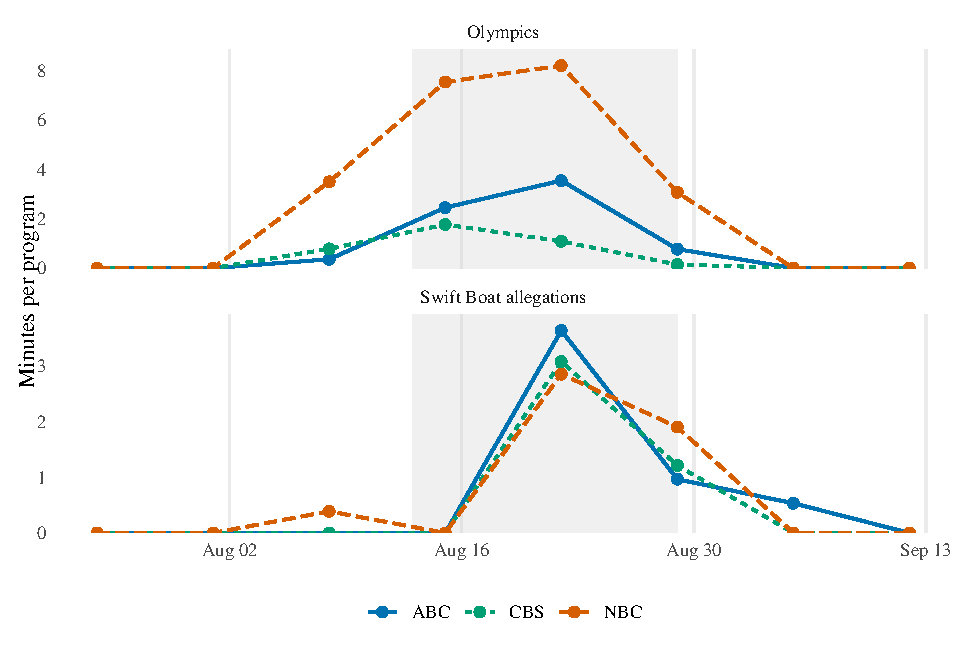
\includegraphics[width=\linewidth]{publicity_coverage.pdf}
\caption{Olympic news expanded while the Swift Boat controversy received coverage. Points average observed evening-news programs within seven-day bins beginning July 22; the final bin has four days. Shading marks August 13--29. Durations include all content within a segment mentioning the topic. Missing programs are omitted, not assigned zero coverage. The two panels have different vertical scales.}
\label{fig:publicity}
\end{figure}

The estimated change in the probability of covering the allegations is \PublicityPresenceEstimate{} percentage points [\PublicityPresenceLower, \PublicityPresenceUpper]. The duration comparison is \PublicityDurationEstimate{} minutes [\PublicityDurationLower, \PublicityDurationUpper]. The latter estimate permits some reduction in attention, but neither measure establishes displacement of the allegations. Weekday-only comparisons, a window ending with the Games, alternative calendar lags, and a broader military-record controversy code retain this distinction between increased Olympic coverage and uncertain scandal crowdout.

\begin{table}[htbp]
\centering\TableStyle
\caption{NBC relative to ABC and CBS during the Olympics}
\label{tab:publicity}
\adjustbox{max width=\linewidth}{\begin{tabular}{lrrr}
\toprule
Outcome & Linear trend & No trend & Days \\
\midrule
Olympics segments (minutes) & 1.2 [-3.0, 5.4] & 4.3 [2.2, 6.5] & 41 \\
Swift Boat coverage (pp) & 2.1 [-28.1, 32.2] & 7.2 [-9.2, 23.6] & 41 \\
Swift Boat segments (minutes) & -0.5 [-1.4, 0.5] & -0.3 [-1.0, 0.3] & 41 \\
Kerry rating: Democrats & -2.5 [-11.7, 6.7] & 0.5 [-4.3, 5.2] & 53 \\
Kerry rating: Republicans & -7.3 [-13.2, -1.4] & -1.6 [-5.8, 2.6] & 53 \\
Kerry rating: Democrats minus Republicans & 4.8 [-5.2, 14.8] & 2.1 [-4.0, 8.1] & 53 \\
\bottomrule
\end{tabular}
}
\caption*{Olympics coefficients and 95\% intervals. Daily outcomes subtract the arithmetic mean of ABC and CBS from NBC. Both specifications include an intercept and a post-Games indicator. Rating comparisons use separate daily means within each party, on a 0--100 scale. The final row directly compares the two partisan contrasts. Bartlett HAC intervals use seven calendar days, an $n/(n-p)$ adjustment, and $t_{n-p}$ critical values. These are exploratory time-series comparisons around one Olympics; intervals are unadjusted for multiple comparisons.}
\end{table}

The National Annenberg Election Survey provides a direct check on the proposed audience mechanism. Its rolling cross-section contains \PublicityInterviews{} interviews during the broadcast window, including \PublicityNetworkViewers{} respondents who identify ABC, CBS, or NBC as their most-watched national network news. We join the original media and awareness questions from the public NAES replication data deposited by \citet{macdonald2025data}. On August 14--16, \AwareNBC\% of NBC viewers reported seeing or hearing about the Swift Boat advertisement, compared with \AwareABC\% of ABC viewers and \AwareCBS\% of CBS viewers. NBC viewers were thus about as aware of the advertisement as viewers of the other networks immediately after the Games opened. Appendix Table~\ref{tab:awareness} reports the pre-opening comparison and denominators. The awareness questions span only August 9--16, so they describe the opening days rather than the full Olympics.

For candidate evaluations, \PublicityPartisanRatings{} ABC, CBS, and NBC viewers identify as Democrats or Republicans and supply a valid Kerry rating. We construct the same daily network contrast separately within each party and estimate the period comparisons in Table~\ref{tab:publicity}. NBC viewers do not show the relative improvement in Kerry's ratings predicted by a simple shielding account. The negative Republican contrast in the trend-adjusted model becomes smaller without the trend; the difference between the partisan contrasts is imprecise. Including partisan leaners likewise changes the estimated partisan difference. These results do not isolate a publicity effect: network preference is measured at the interview, audiences can change, and the conventions and other campaign developments coincide with the window. Audience education also changes across the comparison periods (Appendix Table~\ref{tab:composition}).

The controversy remained visible during a major competing news event. NBC devoted substantial attention to the Olympics while still covering the Swift Boat controversy, and its viewers reported comparable awareness. The evidence supports studying realized coverage and audience knowledge directly rather than treating Olympic overlap alone as a measure of reduced scandal exposure.

\section{Perceived Accountability and Partisan Evaluations}

A November 2013 MTurk survey experiment examines evaluations of partisans who maintain or withdraw their support after controversy \citep{ahler2026}. Respondents read about Obama's health-exchange rollout, Cruz's role in the shutdown controversy, or Rob Ford as a placebo. Within the American stories, the portrayal says that the politician's co-partisans either retained or reduced their support. These are bundled story variants about observed accountability, rather than randomized real-world scandal exposure. Related experiments examine how misconduct and resignation change evaluations of parties \citep{wolsky2022}.

The experiment includes \ExpAssignedN{} assigned partisans, including leaners, of whom \ExpStrongN{} identify strongly with their party. The outcome averages seven favorably oriented trait ratings for each party, excluding patriotism, then compares the respondent's own party with the opposition. We report a rescaled polarization index on a 0--100 scale: $50+(\text{own-party traits}-\text{opposition traits})/2$. A point on this index is therefore twice as large as a point on the raw trait gap and is not an approval or warmth percentage point. The nonresponse-by-strength interaction relative to the Ford placebo is \ExpArchivedInteractionEstimate{} points, with HC3 interval [\ExpArchivedInteractionLower, \ExpArchivedInteractionUpper] and $p=\ExpArchivedInteractionP$.

The more direct question compares out-party nonresponse with out-party response in the same leader's story. We restrict the analysis to respondents passing the pre-treatment attention check and standardize within-party contrasts to the eligible group's party composition. Among the \ExpAttentionStrongN{} strong partisans in the \ExpAttentionN{}-person screened sample, nonresponse increases polarization by \ExpStrongResponseEstimate{} points [\ExpStrongResponseLower, \ExpStrongResponseUpper], $p=\ExpStrongResponseP$ (Table~\ref{tab:experiment}). The corresponding strong-minus-weak interaction is \ExpModerationResponseEstimate{} [\ExpModerationResponseLower, \ExpModerationResponseUpper], $p=\ExpModerationResponseP$. Thus the direct contrast supports polarization among strong partisans, while the evidence that this particular contrast differs by partisan strength is less precise. The placebo-based interaction answers a broader question because the control also changes the leader, controversy, and country. These subgroup analyses are exploratory; probabilities and intervals are unadjusted for multiple comparisons.

\begin{table}[htbp]
\centering\TableStyle
\caption{Polarization after portrayals of out-party nonresponse}
\label{tab:experiment}
\begin{adjustbox}{max width=\textwidth}
\begin{tabular}{llrr}
\toprule
Group & Comparison & Estimate [95\% CI] & $p$ \\
\midrule
Strong & Unchanged vs. control & 10.2 [4.5, 15.9] & $<.001$ \\
Strong & Unchanged vs. response & 5.9 [0.5, 11.2] & .031 \\
Strong minus weak & Unchanged vs. control & 12.2 [5.3, 19.1] & $<.001$ \\
Strong minus weak & Unchanged vs. response & 6.0 [-0.6, 12.6] & .076 \\
\bottomrule
\end{tabular}

\end{adjustbox}
\caption*{Changes on the rescaled 0--100 seven-trait polarization index. Strict pre-treatment attention sample; within-party comparisons standardized to eligible party shares. Strong-minus-weak contrasts use a common sample party composition. Welch--Satterthwaite 95\% intervals and two-sided, unadjusted $p$-values. The full outputs retain unscreened, unstandardized, and HC3 comparisons.}
\end{table}

The direct strong-partisan contrast includes improved evaluations of the respondent's own party: \ExpDirectOwnTraitsEstimate{} trait points [\ExpDirectOwnTraitsLower, \ExpDirectOwnTraitsUpper]. Opposing-party traits change by \ExpDirectOpponentTraitsEstimate{} points [\ExpDirectOpponentTraitsLower, \ExpDirectOpponentTraitsUpper]. The polarization result therefore should not be described solely as a precisely estimated increase in dislike of opponents.

\section{Discussion}

The approval estimates describe modest average losses with a partisan difference. Overall approval, including independents, changes by \OverallEstimate{} points [\OverallLower, \OverallUpper] in the same main specification. That is a meaningful loss of support, although it is much smaller than wholesale abandonment of the politician. The paired partisan contrast indicates somewhat greater protection from co-partisans. It does not establish that most individual scandals have small effects: an average neither describes every event nor counts officials whose careers ended before usable follow-up polls.

Citizens may judge misconduct through their partisan attachments, but an aggregate approval series cannot reveal why they do so. Unequal exposure, different prior beliefs, judgments about the seriousness of an allegation, and continued policy agreement can all produce different responses. Even a well-identified difference in approval penalties would leave those mechanisms unresolved.

The approval evidence favors asymmetric accountability: co-partisans impose a smaller average penalty than opponents in the main specification. Both the directional test and the likelihood comparison support that ordering. Alternative dates, trends, and comparison samples yield smaller differences, making the magnitude of partisan protection an important question for further research.

The survey experiment adds evidence about a downstream consequence. Strong partisans report more polarized trait evaluations when a story depicts opponents retaining support after controversy. That finding concerns assigned portrayals in a particular experiment, while the approval panel concerns observed responses around cataloged events. Together they motivate a connection between perceived accountability and partisan evaluations. They do not identify how frequently real scandal responses cause polarization, or establish that the experimental effect operates entirely through increased dislike of opponents.

\FloatBarrier
\begingroup
\small
\setstretch{1}
\bibliographystyle{plainnat}
\bibliography{references}
\endgroup
\clearpage
\appendix
\section{The Scandal Inventory}

\begin{table}[htbp]
\centering\TableStyle
\caption{Recorded categories and the main analysis}
\label{tab:inventory}
\begin{tabular}{lrr}
\toprule
Recorded category & Coding rows & Main events \\
\midrule
Noncriminal sexual conduct &  6 &  1 \\
Prostitution or solicitation &  3 &  0 \\
Sexual harassment or assault &  2 &  0 \\
Alcohol abuse or DUI &  0 &  0 \\
Illicit drugs &  0 &  0 \\
Corruption or misuse of office & 64 & 12 \\
Racist speech or behavior & 13 &  1 \\
Other inflammatory statements & 19 &  2 \\
Gross incompetence & 25 &  2 \\
\bottomrule
\end{tabular}

\caption*{Coding rows retain the original categories. Several rows can describe the same episode. Main events count the first cataloged event for each retained official; a first row supplies its category. Clean and incomplete rows are excluded from the category counts.}
\end{table}

\begin{table}[htbp]
\centering\TableStyle
\caption{Polling support for dated catalog keys}
\begin{tabular}{lr}
\toprule
Availability after the main window rules & Officials \\
\midrule
Fewer than two polls on both sides & 31 \\
Fewer than two post-event polls & 10 \\
Fewer than two pre-event polls &  4 \\
Included & 18 \\
No matched approval records & 26 \\
\bottomrule
\end{tabular}

\caption*{Counts apply the main twelve-month window, event-month omission, next-event censoring, comparable party definitions, and event-party match. The catalog includes one incomplete Rubio key lacking state and office; it falls in the no-match category. Missing post-event support need not imply resignation or defeat.}
\end{table}
\FloatBarrier

\section{Events, Coverage, and Raw Trajectories}

\begin{table}[htbp]
\centering\TableStyle
\caption{Officials contributing to the main analysis.}
\label{tab:support}
\adjustbox{max width=\linewidth}{\begin{tabular}{lllllrrr}
\toprule
Official & State & Office & Party & Recorded date & Pre & Post & $\Delta$ gap \\
\midrule
Bob Riley & AL & G & R & 2005-11-15 & 6 & 9 & 2.6 \\
Jeff Sessions & AL & S & R & 2009-05-15 & 10 & 6 & 6.3 \\
Jodi Rell & CT & G & R & 2006-03-08 & 10 & 5 & 7.2 \\
Chuck Grassley & IA & S & R & 2009-03-16 & 10 & 6 & 0.4 \\
Ernie Fletcher & KY & G & R & 2006-05-12 & 12 & 9 & -2.9 \\
Jim Bunning & KY & S & R & 2009-02-23 & 10 & 9 & -4.8 \\
John Kerry & MA & S & D & 2006-11-01 & 12 & 12 & -7.2 \\
Norm Coleman & MN & S & R & 2008-10-30 & 10 & 2 & 22.6 \\
Matt Blunt & MO & G & R & 2008-01-10 & 12 & 9 & -0.3 \\
Kit Bond & MO & S & R & 2008-11-30 & 10 & 11 & -4.8 \\
Conrad Burns & MT & S & R & 2006-03-27 & 10 & 4 & 6.7 \\
Byron Dorgan & ND & S & D & 2005-12-05 & 7 & 10 & 4.1 \\
Frank Lautenberg & NJ & S & D & 2006-02-28 & 9 & 8 & -4.2 \\
Bill Richardson & NM & G & D & 2008-12-15 & 9 & 9 & -2.8 \\
Pete Domenici & NM & S & R & 2007-03-05 & 11 & 12 & 4.3 \\
Bob Taft & OH & G & R & 2005-08-17 & 3 & 12 & -2.1 \\
Bill Frist & TN & S & R & 2005-09-23 & 4 & 8 & 4.9 \\
Maria Cantwell & WA & S & D & 2006-10-02 & 12 & 11 & 7.2 \\
\bottomrule
\end{tabular}
}
\begin{minipage}{\linewidth}\footnotesize
\emph{Note}: G denotes governor and S senator. Pre and post count politician-poll observations after the window, complete-case, party, and later-event restrictions. Dates are the first cataloged events, not necessarily the first public revelations. The final column is the unadjusted within-official post-minus-pre change in the approval gap. It is descriptive and has no trend adjustment.
\end{minipage}
\end{table}

Raw gap changes vary substantially across officials, from \EventMinChange{} to \EventMaxChange{} points. Figure~\ref{fig:paths} shows the observed trajectories on common axes. The sparse and uneven timing is visible; the curves connect observed polls and do not interpolate missing survey evidence for estimation.

\clearpage
\begin{figure}[p]
\centering
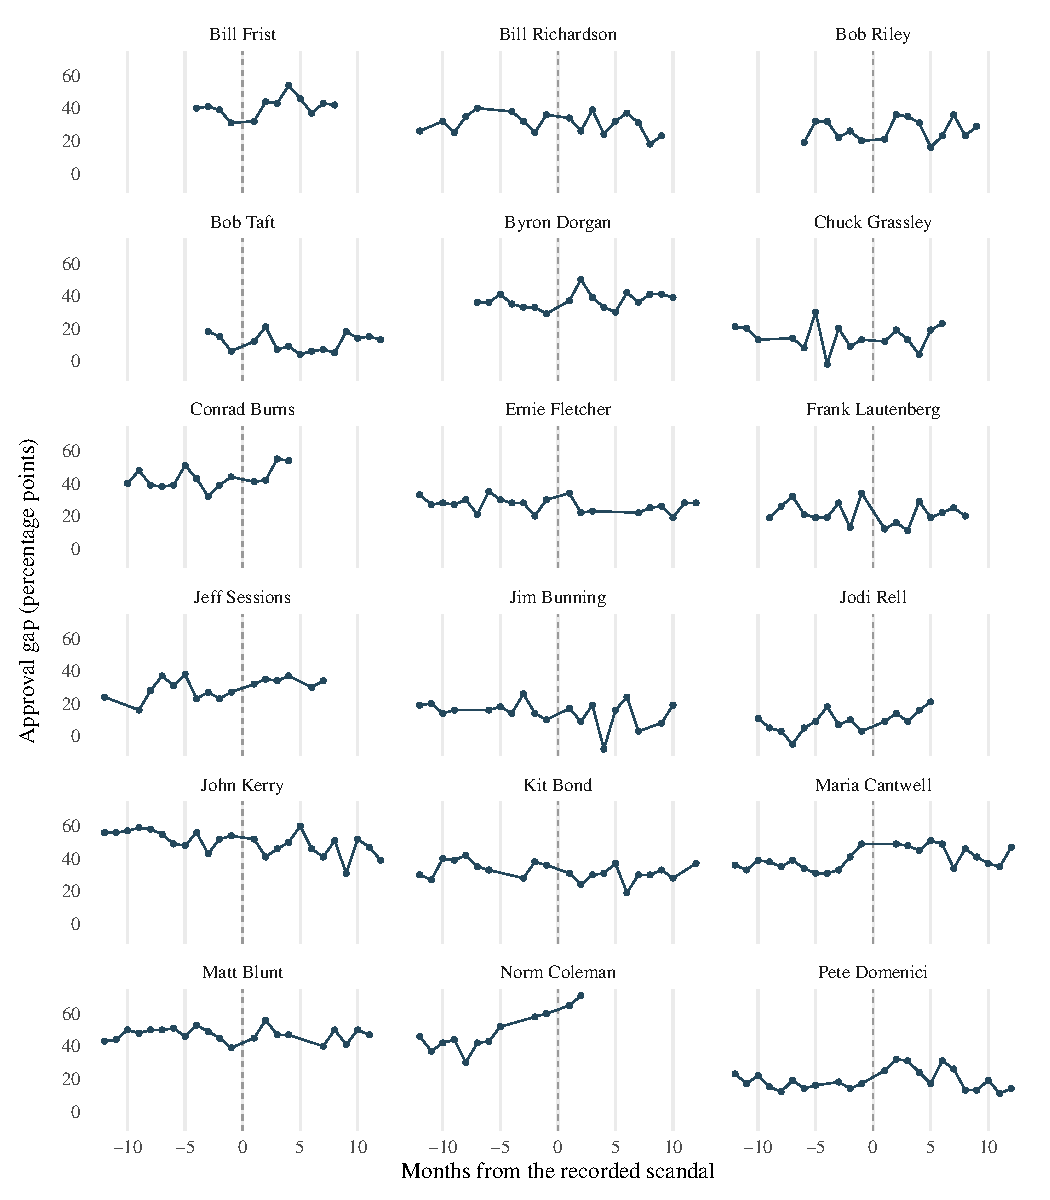
\includegraphics[width=.94\linewidth,height=.86\textheight,keepaspectratio]{event_paths.pdf}
\caption{Observed co-partisan minus opposing-partisan approval by official. Points are aggregate poll differences in percentage points; lines connect observed polls. The vertical reference marks the recorded event month, which is omitted. Common axes permit comparison across officials. These are raw data, not estimated causal response curves.}
\label{fig:paths}
\end{figure}
\clearpage
\section{Exploratory Subgroups}
\begin{table}[htbp]
\centering\TableStyle
\caption{Partisan differences within exploratory subgroups.}
\label{tab:subgroups}
\begin{tabular}{lrrrrr}
\toprule
Subgroup & Gap change & 95\% CI & Officials & States & df \\
\midrule
Republicans & 3.7 & [-0.8, 8.2] & 13 & 10 & 7.5 \\
Democrats & 1.8 & [-7.1, 10.6] & 5 & 5 & 3.9 \\
Governors & 1.9 & [-2.1, 5.9] & 6 & 6 & 5.0 \\
Senators & 3.8 & [-1.2, 8.8] & 12 & 12 & 10.8 \\
Corruption & 4.0 & [-0.1, 8.0] & 12 & 10 & 7.5 \\
Other & 1.6 & [-5.0, 8.2] & 6 & 6 & 5.0 \\
\bottomrule
\end{tabular}

\begin{minipage}{\linewidth}\footnotesize
\emph{Note}: Separate versions of the main model within each subgroup. CR2 state-clustered 95\% confidence intervals with Satterthwaite degrees of freedom. These are conditional associations, with no multiplicity adjustment. Differences in statistical significance across rows do not test differences between subgroups.
\end{minipage}
\end{table}

\section{Publicity, Awareness, and Audience Composition}

The broadcast analysis uses archive titles, abstracts, and segment durations. The source ledger retains each program and segment identifier, download URL, content hash, and topic decision. Olympic coverage concerns the Games, athletes, and host setting; incidental references within campaign stories are excluded. Three substantive segments discuss the allegations without using the phrase ``Swift Boat''; these enter the principal code after review of their abstracts. A broader code adds military-record attacks during the Republican convention. The downloaded records also include a separate 2008 window around the Troopergate report; those programs do not enter the 2004 comparisons.

NAES observations receive equal weight, following the survey's original unweighted release. Network preference identifies the national evening-news program watched most often among respondents reporting some network-news viewing in the preceding week. It is contemporaneous, and does not measure exclusive exposure to that network or exposure before the Games. Favorability codes outside 0--10, don't-know responses, and unasked questions remain missing for the relevant outcome. Strict Democrats and Republicans define the principal party comparison; an alternative includes partisan leaners. Each day receives equal weight in the network-gap regressions, and ABC and CBS receive equal weight in the comparison network average.

\begin{table}[htbp]
\centering\TableStyle
\caption{Awareness of the Swift Boat advertisement around the Olympics opening}
\label{tab:awareness}
\begin{tabular}{llrrrr}
\toprule
Network & Interview dates & $N$ & Seen & Heard only & Aware (\%) \\
\midrule
ABC & August 9--12 & 189 & 61 & 49 & 58.2 \\
ABC & August 14--16 & 169 & 71 & 40 & 65.7 \\
CBS & August 9--12 & 143 & 60 & 34 & 65.7 \\
CBS & August 14--16 & 100 & 46 & 21 & 67.0 \\
NBC & August 9--12 & 227 & 90 & 56 & 64.3 \\
NBC & August 14--16 & 172 & 73 & 42 & 66.9 \\
\bottomrule
\end{tabular}

\caption*{Unweighted NAES respondents naming ABC, CBS, or NBC as their most-watched national network news and answering the awareness question. ``Aware'' combines having seen the advertisement and having heard of it. August 13 interviews are omitted because interview times cannot establish exposure to that evening's coverage. The remaining interviews span four days before and three days after the opening; no time-series significance claim is made from this short comparison.}
\end{table}

\begin{table}[htbp]
\centering\TableStyle
\caption{Audience composition during the Olympics}
\label{tab:composition}
\adjustbox{max width=\linewidth}{\begin{tabular}{llrr}
\toprule
Audience characteristic & Specification & Change & 95\% interval \\
\midrule
Mean age (years) & Linear trend & -1.71 & [-3.53, 0.11] \\
Mean age (years) & No trend & 0.18 & [-0.96, 1.32] \\
College degree (percentage points) & Linear trend & 2.48 & [-5.50, 10.46] \\
College degree (percentage points) & No trend & 2.56 & [-1.30, 6.43] \\
Identify as Democrats (percentage points) & Linear trend & -5.13 & [-14.33, 4.06] \\
Identify as Democrats (percentage points) & No trend & -4.85 & [-8.76, -0.93] \\
Mean education category (1--9) & Linear trend & 0.44 & [0.15, 0.73] \\
Mean education category (1--9) & No trend & 0.29 & [0.12, 0.46] \\
Women (percentage points) & Linear trend & -3.98 & [-11.93, 3.97] \\
Women (percentage points) & No trend & -5.01 & [-10.29, 0.27] \\
NBC share among ABC/CBS/NBC viewers & Linear trend & -0.68 & [-4.08, 2.72] \\
NBC share among ABC/CBS/NBC viewers & No trend & 1.26 & [-0.60, 3.12] \\
\bottomrule
\end{tabular}
}
\caption*{Olympics coefficients from daily NBC-minus-mean-ABC/CBS composition comparisons. The final characteristic instead measures NBC's share of all three networks' respondents. Specifications, calendar HAC intervals, and equal-day weighting follow Table~\ref{tab:publicity}. Education runs from eighth grade or less to a postgraduate degree; it is an ordinal category, not years of schooling. College degree denotes a four-year degree or higher. All valid network viewers contribute, including independents. These comparisons describe audience changes rather than correcting selection into network viewing.}
\end{table}
\FloatBarrier

\section{Sources and Event Measurement}
\label{sec:limits}

The approval series combines monthly records with SurveyUSA polls that retain fieldwork dates. Reported percentages agree across overlapping source records. Exact partisan subgroup denominators are unavailable throughout the series, so the analysis weights politician-poll observations equally. Selective cessation of polling after resignation or defeat can limit observation of the most consequential scandals.

The episode ledger links each allegation and later development to a dated source. Publication dates, alleged conduct dates, and dates of subsequent investigations or clearances remain separate. Uncertain dates are recorded as intervals. External inventories from \citet{preuss2024,nyhan2017} provide additional chronologies under their respective first-report and media-recognition definitions. They are joined by person, state, and office, with original date definitions retained. The broader historical catalog supplies the event sample analyzed here.

The replication materials include the original source records, event-source links, alternative timing specifications, and code for all reported estimates and exhibits.

\end{document}
